\section{Експериментальні результати}\label{section2.1}

Для перевірки гіпотез на практиці було написано набір Python скриптів.
За основу взято відомий датасет текстур Бродатца \cite{brodatz} із фотографіями у відтінках сірого у однорідному освітленні.
Цей датасет використовується в тому числі для сумісності результатів із іншими науковими роботами.
Спочатку з оригінального датасету утворено тренувальні та тестові вибірки у потрібному форматі.
Далі проведено перевірку деяких сформульованих в роботі статистичних гіпотез для цієї вибірки.
Потім підготовлено статистичну модель для класифікації текстур декількома методами і оцінено їх ефективність.

\subsection{Підготовка даних}\label{section2.1a}

\begin{figure}[h]
    \centering
    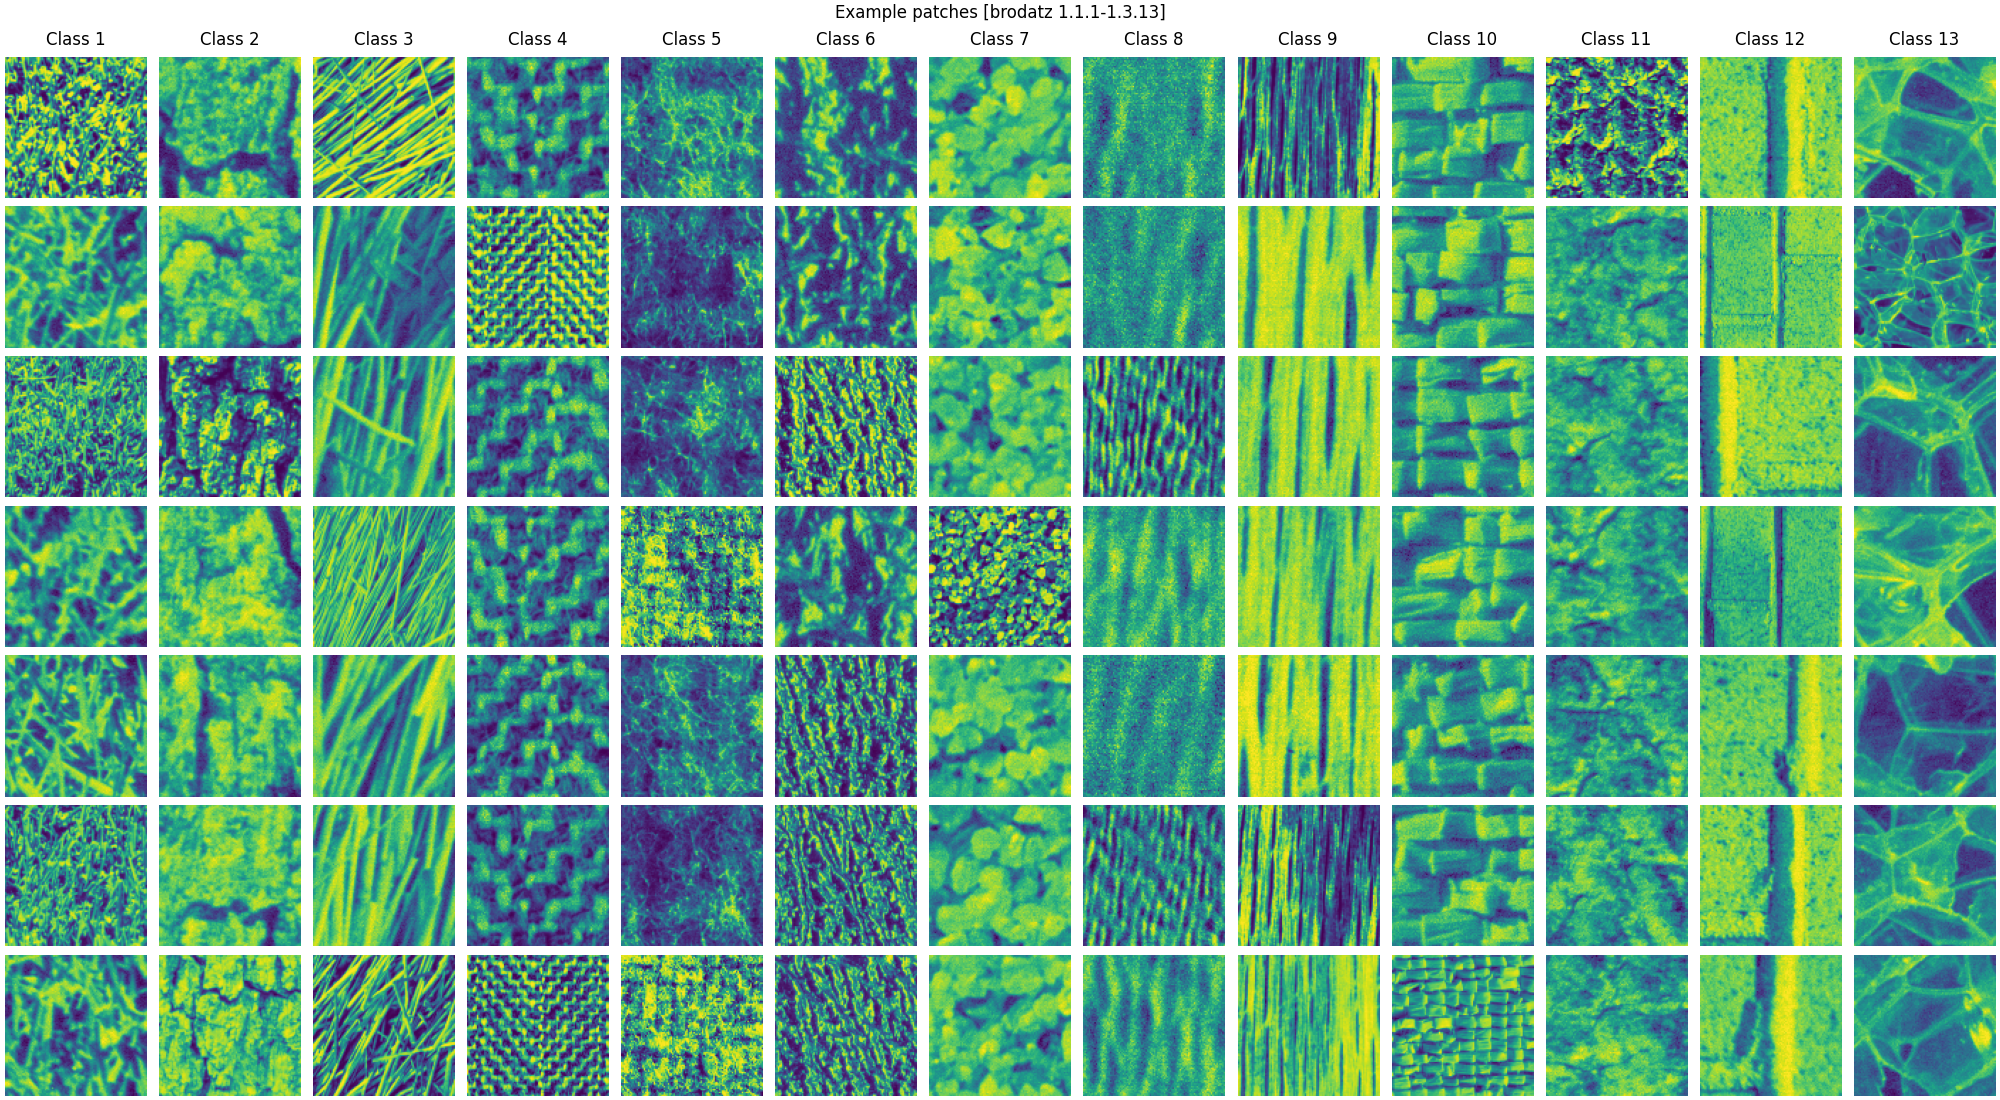
\includegraphics[width=0.95\textwidth]{img/example_classes.png}
    \caption{
        Приклад патчів 100x100 у відтінках сірого, утворених з датасету текстур Бродатца; для кожного з типів текстур у наборі.
        Візуалізовано у псевдокольорах.
    }
    \label{fig:brodatz-showcase}
\end{figure}

У роботі використано перші три частини датасета Бродатца, які містять фотографії текстур у відтінках сірого у великому наближенні, всього 39 різних фотографій.
Датасет включає як однорідні та регулярні текстури (цегла, тканина), так і псевдорегулярні (дерево, кора, трава, сіно, шкіра). 
Кожна частина складається з 13-ти фотографій різних текстур (природних та штучних), при чому послідовність текстур повторюється між частинами. 
Зображення у перших двох частинах мають розміри 512 на 512 пікселів. 
Третя частина містить фотографії в іншому масштабі та у розмірі 1024 на 1024 пікселів.
Оригінальні фотографії розрізано на неперетинні квадратні частини (патчі) розміром 100 на 100 пікселів (ігноруючи залишкові пікселі).
Кожному патчу призначено дві мітки: номер текстури (1-13), та номер фотографії цієї текстури, з якого патч походить (1-3).

Таким чином, робоча вибірка містить по 350 патчів з першої та другої частин, і 1300 патчів з третьої частини; всього 1950 елементів вибірки.
Всі текстури представлені у вибірці збалансовано, кожна має по 150 представників.

\subsection{Вибір LBP дескрипторів}\label{section2.1b}

У якості дескрипторів у роботі будуть дескриптори LBP із різними параметрами R та P, у стандартному та "рівномірному" варіантах.
Для сумісності результатів із попередніми дослідженнями \cite{ojala2002,fastlbp2024}, обрано наступні параметри:
(R=1,P=8, 'default'), (R=2,P=12,'default'), (R=1,P=8, 'uniform'), (R=2,P=12,'uniform'), (R=3,P=24,'uniform'), (R=5,P=36,'uniform').

Для кожного патчу обчислено декілька векторів ознак, по вектору для кожного з обраних дескрипторів 



\subsection{Перевірка статистичних гіпотез}\label{section2.1c}

\subsection{Результати класифікації}\label{section2.1d}

